\sectionSlide{Cfront era}{binario}{\paperwidth}{b}


\slide{The C++ Programming language - 1st edition (1983)}{
    %NOTE: Tell that Bjarne wrote this book to show people how to code in C++. They were reluctant to write Object Oriented code. They were skeptical. How do you learn anything new in programming? I guess that you do the same thing as I do. There are 2 schools.
    \only<1>{
        \centering 
        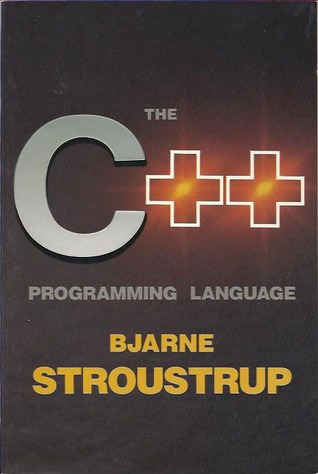
\includegraphics[height=0.8\paperheight]{the-cpp-programming-language}
    }
    %NOTE: First is changing things and seeing what happens. It's easy. In that way I can learn many things.
    \only<2>{
        \centering 
        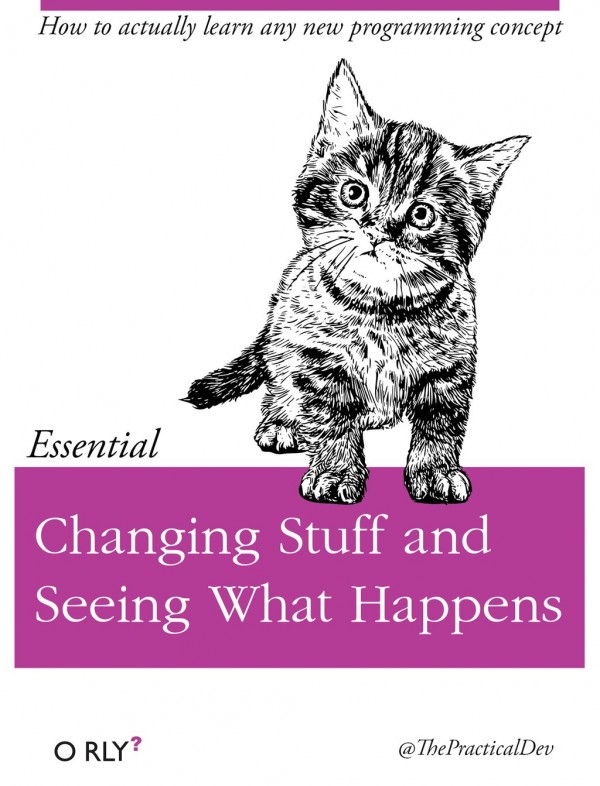
\includegraphics[height=0.8\paperheight]{changing-stuff-and-seeing-what-happens}
    }
    %NOTE: The other - just trying some stuff until it works
    \only<3>{
        \centering 
        
\includegraphics[height=0.8\paperheight]{trying-stuff-until-it-works}
    }
    %NOTE: These are really good books. I recommend them both.
    %NOTE: But the interesting fact is the opening line of that book. Bjarne put this text there:
    \begin{alertblock}<4->{The opening line}
		\st{``C++ is a general purpose programming language designed to make programming more enjoyable for the serious programmer''} % TODO: zostawić przekreślone
	\end{alertblock}
    %NOTE: But reviewers weren't happy with that and couldn't believe that it was the main reason. Opening line was changed to below:
    \begin{block}<5>{The opening line}
        \textit{``C++ was designed primarily so that the author and his friends would not have to program in assembler, C, or various modern high-level languages. Its main purpose is to make writing good programs easier and more pleasant for the individual programmer''}
    \end{block}
    %NOTE: And it was accepted without any problems
}


\timeSlide{C84 and Cfront}{
    \itemstep{
        \item C with Classes got new name - C84
        \item A few months later C84 got a new name - C++
        \item First C++ compiler - Cfront
        \begin{itemize}
            \item Originally written in... C with Classes
            \item Transpiler to C code
            \item Portability matters
            \item C++ versions were named after Cfront releases
        \end{itemize}
    }
 
}{
    \draw[thin,blue]
    (0.5, 0) node(l1979)[anchor=west] {1979 C with Classes}
    (0.5,-0.4) node(l1981)[anchor=west] {1981 New features}
    (0.5,-0.7) node(l1983)[anchor=west] {1983 1st std lib}
    (0.5,-1.1) node(l1984)[anchor=west,fill=green!20,rounded corners] {\textbf{1984} C84/C++};
    
    \draw[]
    (1979) -- (l1979)
    (1981) -- (l1981)
    (1983) -- (l1983)
    (1984) -- (l1984);
}


\timeSlide{Cfront 1.0}{
    New features:
    \enumstep{
        \item virtual functions
        \item function name and operator overloading
        \item references
        \item constants (const)
        \item new and delete operators
        \item improved type checking
        \item scope resolution operator (::)
        \item BCPL-style comment terminated by end-of-line
    }
    
}{
    \draw[thin,blue]
    (0.5, 0) node(l1979)[anchor=west] {1979 C with Classes}
    (0.5,-0.4) node(l1981)[anchor=west] {1981 New features}
    (0.5,-0.7) node(l1983)[anchor=west] {1983 1st std lib}
    (0.5,-1.0) node(l1984)[anchor=west] {1984 C84/C++}
    (0.5,-1.4) node(l1985)[anchor=west,fill=green!20,rounded corners] {\textbf{1985} Cfront 1.0};
    
    \draw[]
    (1979) -- (l1979)
    (1981) -- (l1981)
    (1983) -- (l1983)
    (1984) -- (l1984)
    (1985) -- (l1985);
}


\slide{Example code in C++ 1.0}{
    Virtual functions:
    \only<1>{\lstinputlisting{"src/cfront1_virtual.hpp"}}
    %NOTE: Virtual meant abstract
    \only<2>{\highlightedListing{7}{8}{"src/cfront1_virtual.hpp"}}
}


\slide{Example code in C++ 1.0}{ %TODO: zwiększyć czcionkę
	%TODO: Remove this slide? Only say about overload keyword.
	\Large
    Overloaded functions:
    \only<1>{\lstinputlisting{"src/cfront1_overload.hpp"}}
%    \only<2>{\highlightedListing{1}{1}{"src/cfront1_overload.hpp"}}
}


\slide{Example code in C++ 1.0}{
    New and delete operators:
    Because you want to write that:
    \lstinputlisting[linerange={1-1}]{"src/cfront1_new.hpp"}\pause
    Instead of that:
    \lstinputlisting[linerange={3-5}]{"src/cfront1_new.hpp"}
}


\slide{Example code in C++ 1.0}{
	%TODO: Think about removing this slide
    Improved type checking: % TODO: zaznaczyć 3 kropki na zielono
    \lstinputlisting{"src/cfront1_printf.hpp"}
}


\timeSlide{Cfront 1.1 (1986) \& Cfront 1.2 (1987)}{
    New features:
    \begin{enumerate}
        \item bug fixes
        \item pointers to members
        \item protected members
    \end{enumerate}
    
}{
    \draw[thin,blue]
    (0.5, 0) node(l1979)[anchor=west] {1979 C with Classes}
    (0.5,-0.4) node(l1981)[anchor=west] {1981 New features}
    (0.5,-0.7) node(l1983)[anchor=west] {1983 1st std lib}
    (0.5,-1.0) node(l1984)[anchor=west] {1984 C84/C++}
    (0.5,-1.4) node(l1985)[anchor=west,fill=green!20,rounded corners] {\textbf{1985} Cfront 1.0};
    
    \draw[]
    (1979) -- (l1979)
    (1981) -- (l1981)
    (1983) -- (l1983)
    (1984) -- (l1984)
    (1985) -- (l1985);
}


\timeSlide{Cfront 2.0}{
    New features:
    \begin{enumerate}
        \item multiple inheritance
        \item type-safe linkage
        \item better resolution of overloaded functions
        \item recursive definition of assignment and initialization
        \item defined memory management
        \item abstract classes
        \item static member functions
        \item const member functions
        \item overloading of operator ->
    \end{enumerate}
    
}{
    \draw[thin,blue]
    (0.5, 0) node(l1979)[anchor=west] {1979 C with Classes}
    (0.5,-0.4) node(l1981)[anchor=west] {1981 New features}
    (0.5,-0.7) node(l1983)[anchor=west] {1983 1st std lib}
    (0.5,-1.0) node(l1984)[anchor=west] {1984 C84/C++}
    (0.5,-1.3) node(l1985)[anchor=west] {1985 Cfront 1.0}
    (0.5,-1.7) node(l1989)[anchor=west,fill=green!20,rounded corners] {\textbf{1989} Cfront 2.0};
    
    \draw[]
    (1979) -- (l1979)
    (1981) -- (l1981)
    (1983) -- (l1983)
    (1984) -- (l1984)
    (1985) -- (l1985)
    (1989) -- (l1989);
}


\timeSlide{Cfront 3.0}{
    New features:
    \begin{enumerate}
        \item namespaces
        \item templates
        \item exceptions?	%NOTE: See BaSz presentation on exceptions
        \item nested classes
    \end{enumerate}
    
}{
    \draw[thin,blue]
    (0.5, 0) node(l1979)[anchor=west] {1979 C with Classes}
    (0.5,-0.4) node(l1981)[anchor=west] {1981 New features}
    (0.5,-0.7) node(l1983)[anchor=west] {1983 1st std lib}
    (0.5,-1.0) node(l1984)[anchor=west] {1984 C84/C++}
    (0.5,-1.3) node(l1985)[anchor=west] {1985 Cfront 1.0}
    (0.5,-1.6) node(l1989)[anchor=west] {1989 Cfront 2.0}
    (0.5,-2.0) node(l1991)[anchor=west,fill=green!20,rounded corners] {\textbf{1991} Cfront 3.0};
    
    \draw[]
    (1979) -- (l1979)
    (1981) -- (l1981)
    (1983) -- (l1983)
    (1984) -- (l1984)
    (1985) -- (l1985)
    (1989) -- (l1989)
    (1991) -- (l1991);
}


\timeSlide{Cfront 4.0}{
    New features:
    \begin{enumerate}
        \item Exception handling
    \end{enumerate}
    
}{
    \draw[thin,blue]
    (0.5, 0) node(l1979)[anchor=west] {1979 C with Classes}
    (0.5,-0.4) node(l1981)[anchor=west] {1981 New features}
    (0.5,-0.7) node(l1983)[anchor=west] {1983 1st std lib}
    (0.5,-1.0) node(l1984)[anchor=west] {1984 C84/C++}
    (0.5,-1.3) node(l1985)[anchor=west] {1985 Cfront 1.0}
    (0.5,-1.6) node(l1989)[anchor=west] {1989 Cfront 2.0}
    (0.5,-2.0) node(l1991)[anchor=west] {1991 Cfront 3.0}
    (0.5,-2.4) node(l1993)[anchor=west,fill=green!20,rounded corners] {\textbf{1993} Cfront 4.0};
    
    \draw[]
    (1979) -- (l1979)
    (1981) -- (l1981)
    (1983) -- (l1983)
    (1984) -- (l1984)
    (1985) -- (l1985)
    (1989) -- (l1989)
    (1991) -- (l1991)
    (1993) -- (l1993);
}


\slide{Cfront RIP}{
	\centering
	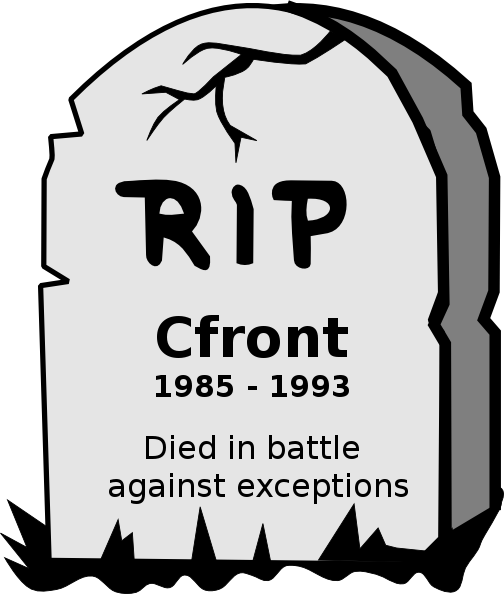
\includegraphics[height=0.8\paperheight]{rip-tombstone}
}


\slide{Cfront - summary}{
	\itemstep{
		\item Years of development: 1985-1993
		\item Compiler's frontend
		\item Translated C++ to C (free portability)
		\item Explosion of interest:
			\begin{itemize}
				\item commercial release in 1885
				\item from \textbf{500 users in 1985}...
				\item to \textbf{over 1 500 000 users in 1993}!
				\item exponential growth!
			\end{itemize}
		\item Many new features added
		\item New approach to exceptions was impossible to be added
	}
}